\documentclass{article}
\usepackage{setspace,tikz}
\usepackage[text={6.5in,8.5in},centering]{geometry}
\geometry{verbose,a4paper,tmargin=2.4cm,bmargin=2.4cm,lmargin=2.4cm,rmargin=2.4cm}
\usepackage{graphicx,amsmath,cases,multirow,appendix,graphicx,xcolor}

\setlength\parindent{0pt}

\newcommand{\note}[1]{\colorbox{gray!20}{#1}}
\newcommand*\circled[1]{\tikz[baseline=(char.base)]{
            \node[shape=circle,draw,inner sep=2pt] (char) {#1};}}

\begin{document}


\noindent\makebox[\textwidth][c]{\Large\bfseries Lecture 2 - Density-independent deterministic growth}

\rule[0.5ex]{\linewidth}{1pt}
\textbf{Announcements}: \\
Today - Paper discussion until $\approx$ 10:45, then 5 min break, then lecture.\\
Next class: Bring laptop \& R, having read readings \& problem set \\
Will provide intro to R, then start problem set together.\\

\textbf{Today's concepts}: \\
Geometric vs. Exponential growth \\
Discrete vs. Continuous (Difference vs. Differential equations) \\
Population vs. Per capita rates of change \\
Simulations vs. Analytical Solutions

\rule[0.5ex]{\linewidth}{1pt}
Overview:
\begin{center}
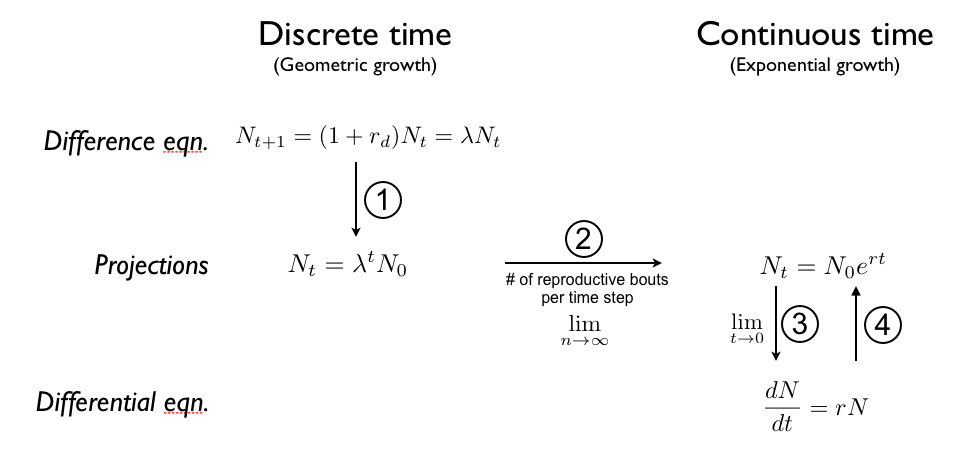
\includegraphics[width=12cm]{figs/EqnConnections.png}
\end{center}
\rule[0.5ex]{\linewidth}{1pt}

\circled{1}
Simplest possible model: Discrete time difference equation:  
\begin{equation*}
N_{t+1}=N_t+B-D+I-E
\end{equation*}
\begin{center}
$B$-Total births; $D$-Total deaths; $I$-Immigration; $E$-Emigration
\end{center}

Let: $\;\;\;\ I=E$, $B=b_d N$, $D=d_d N$.
\begin{center}
	$b_d$ - births per individual; \\$d_d$ - deaths per individual i.e. probability of individual dying per time-step 
\end{center}

Thus:
\begin{equation*}
	N_{t+1}=N_t+(b_d-d_d)N_t=(1+b_d-d_d)N_t=(1+r_d)N_t=\lambda N_t
\end{equation*}

$\lambda$ - “finite rate of increase” - per capita rate of growth if population is growing geometrically\\ 
$r_d$ - discrete growth factor/increment (Ted Case writes this as $R$).

\vspace{1cm}

\note{Draw $N(t)$ vs. $t$ on arithmetic scale on board in steps}
\begin{center}
$N(0)=1, \lambda=2 \implies N(t)=1,2,4,8,16,32,... \implies \text{\textbf{Geometric growth}}$
\end{center}
NOTE:  Not just doubling!  $\lambda$ can be any number!

\note{Then draw on log-scale.}
\begin{center}
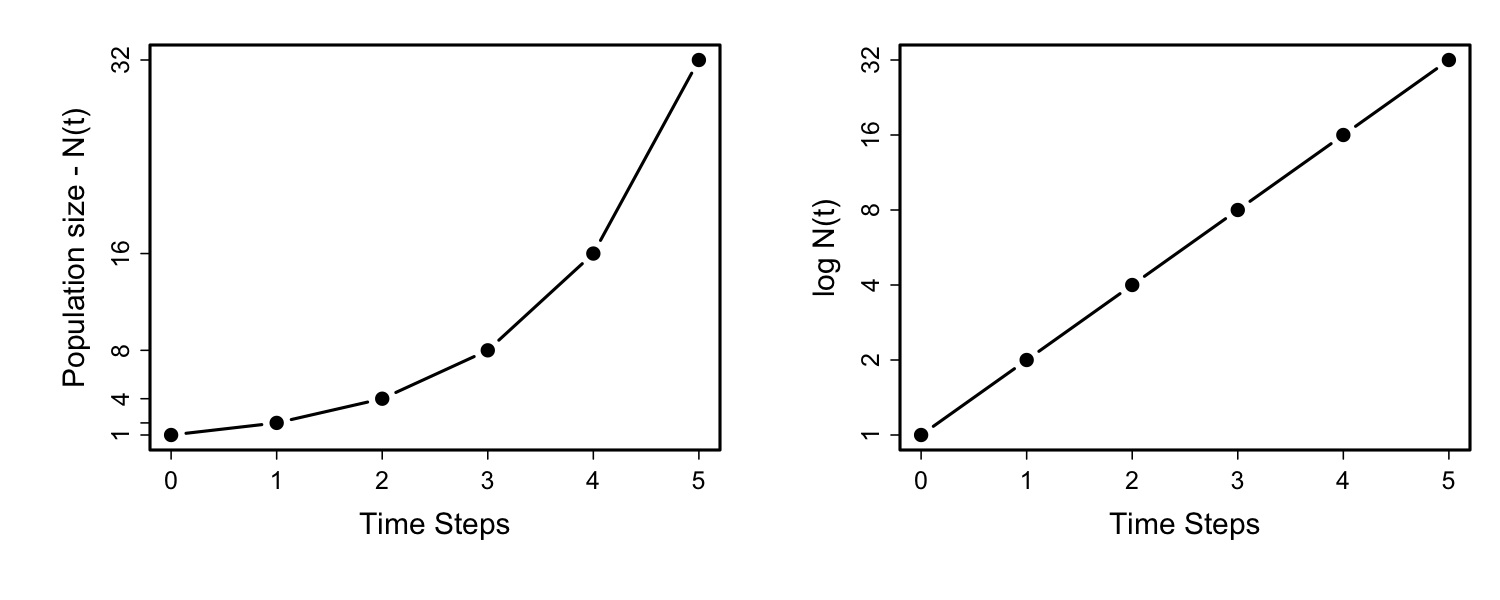
\includegraphics[width=8cm]{figs/image}
\end{center}

\note{Show R plots}

\note{Q:}  What happens if we start at different population size at same lambda?

\note{Add points for N(0)=2 on drawing. Plot in R}
\begin{center}
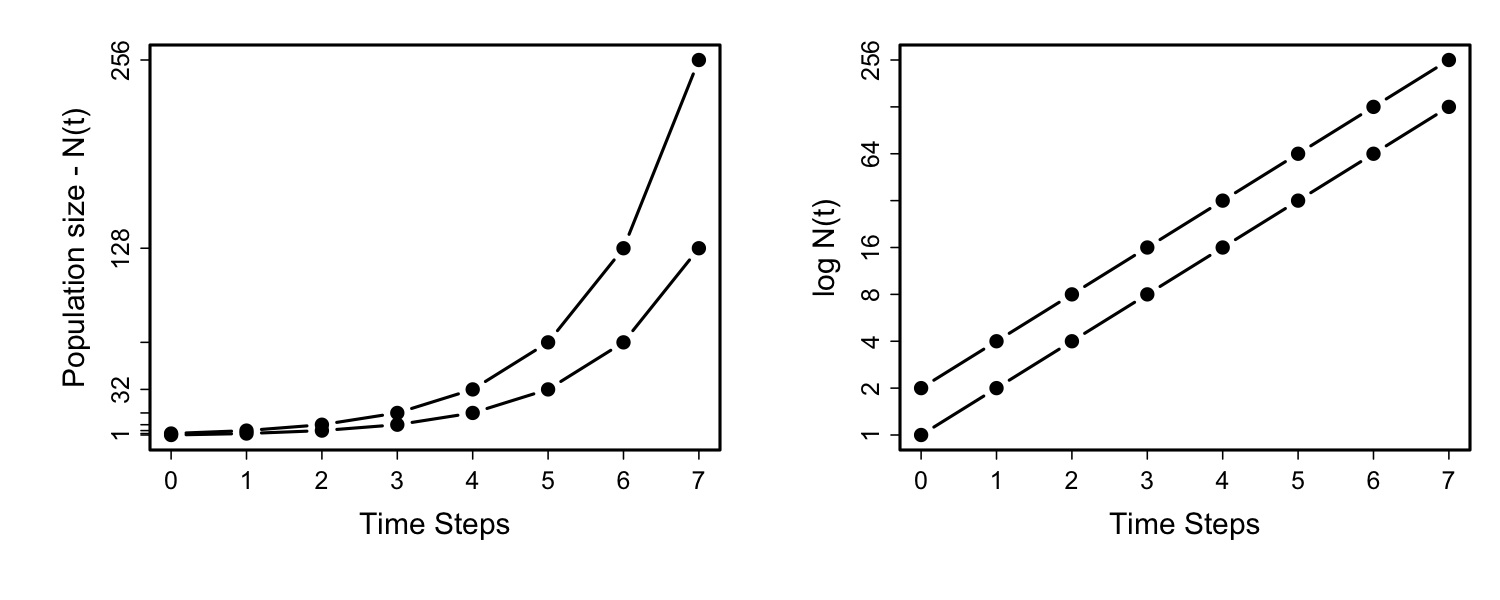
\includegraphics[width=8cm]{figs/image0}
\end{center}

\note{Q:}  Why linear on log-scale?

\note{A:} On log-scale, products become sums, ratios become differences:

\begin{align*}
& y=a \cdot b & y=\frac{a}{b}  & \\
 & log(y)=log(a \cdot b) = log(a) + log (b) & log(y)=log\left(\frac{a}{b}\right )=log(a)-log(b)&
\end{align*}

\note{Q:} Why do we call this density-independent population growth? 

\note{A:} Density independence of \emph{per capita} growth rate

\note{Show plot of $\lambda=\frac{N_{t+1}}{N_t}$ vs. $N_t$}
\begin{center}
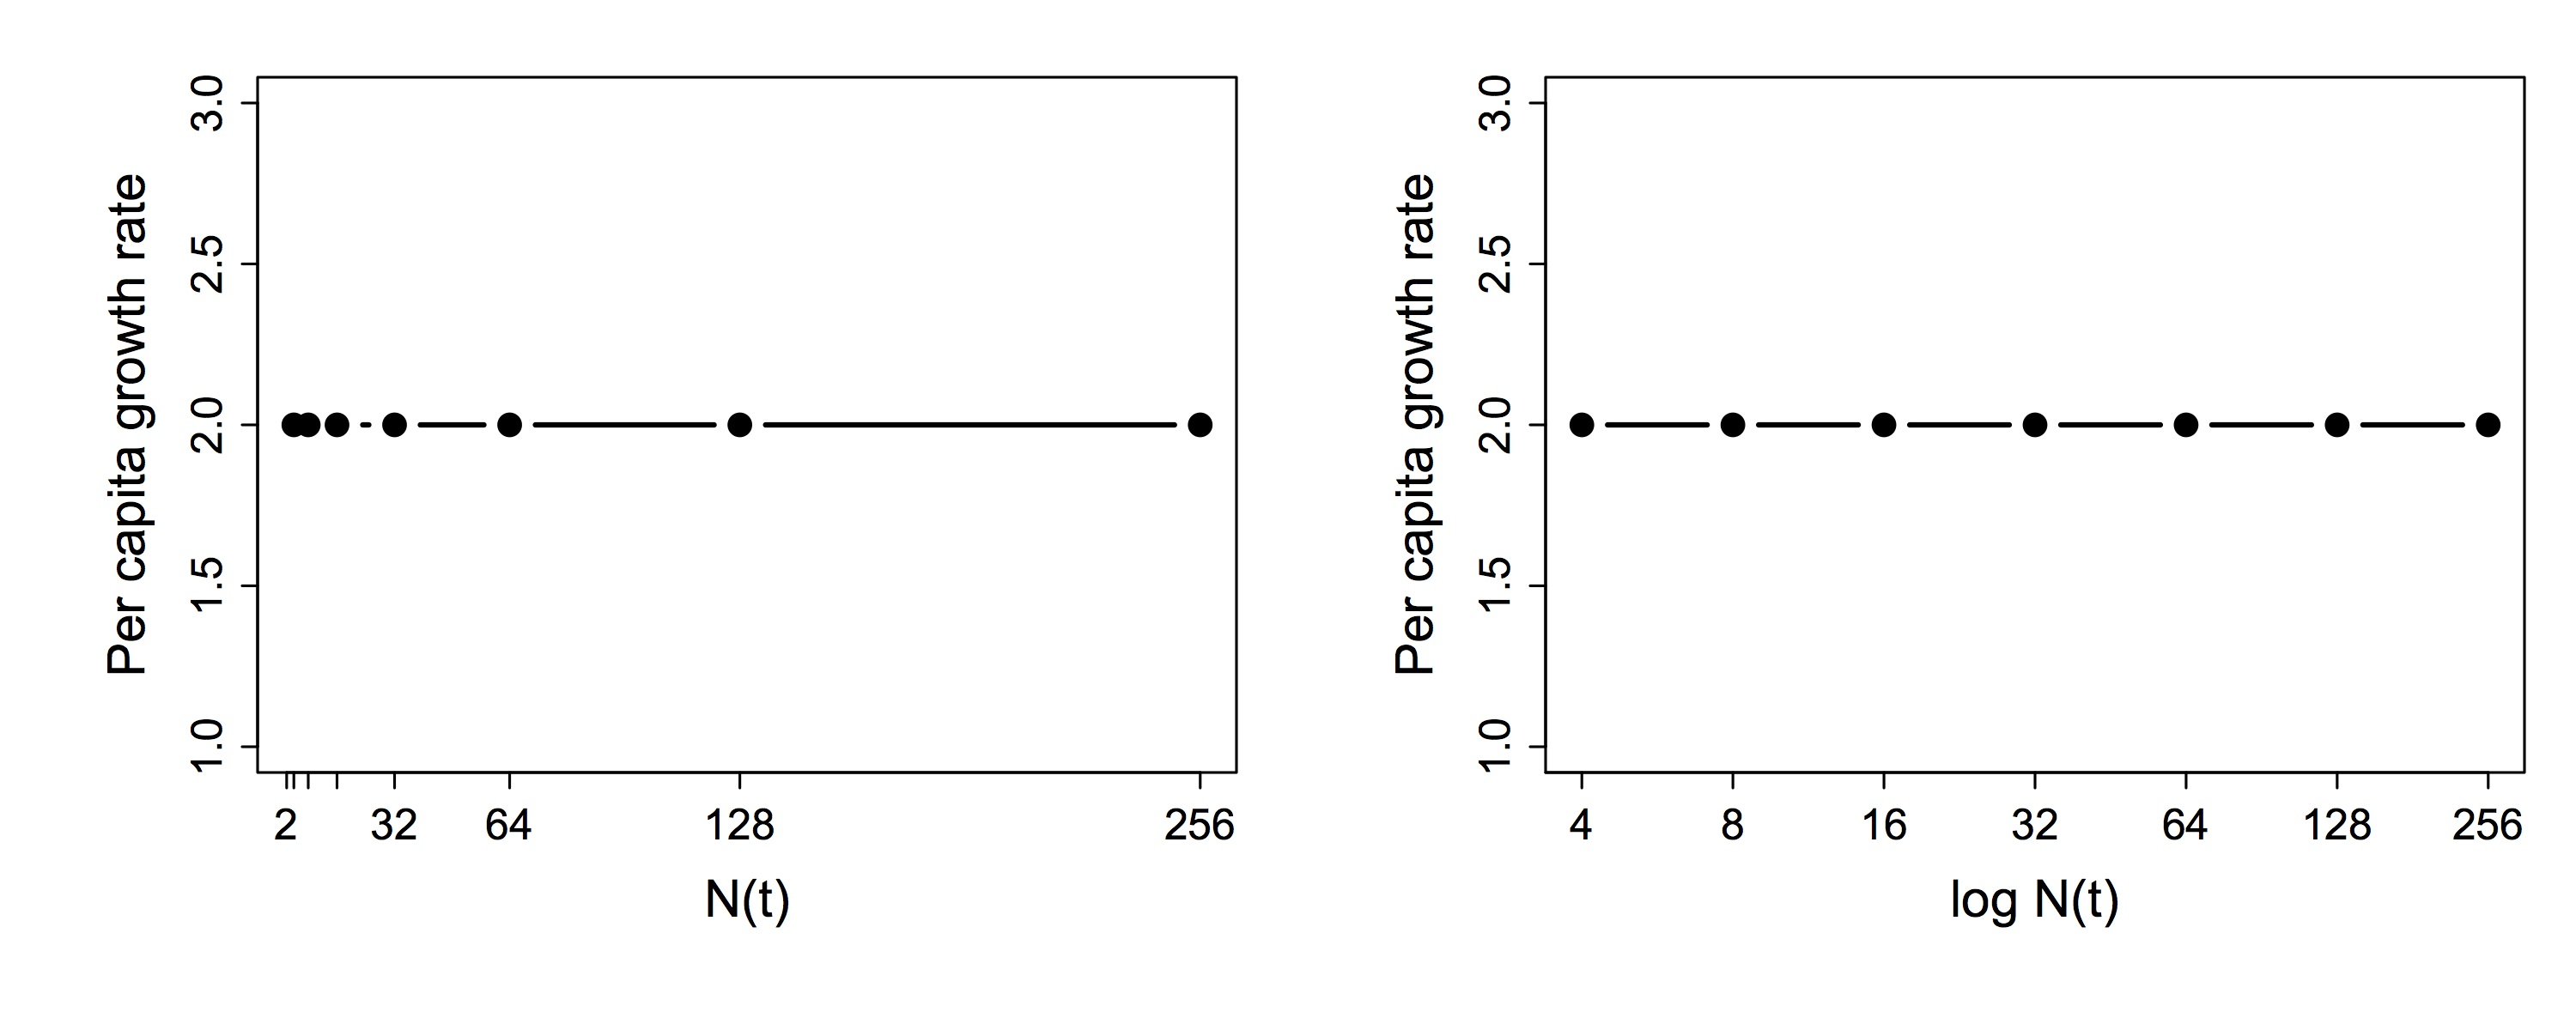
\includegraphics[width=10cm]{figs/image1}
\end{center}
Want to predict $N(T)$:  Analytical solution of $\lambda...(\lambda(\lambda N_0)) = \lambda^T N_0$


\note{Q:}  What have we assumed?

\note{A:}	List includes:
\begin{itemize}
	\item	synchronous discrete reproduction
	\item	constant (non-stochastic = deterministic) growth rate
	\item	no density-dependence
\end{itemize}

Note:\\
Will go back and forth between calculating per capita growth as either $\frac{N_{t+1}}{N_t}$ or $\frac{(N_{t+1}-N_t)}{N_t}$.

Why? Because:
\begin{align*}
& N_{t+1} =\lambda N_t \;\; 
\implies \lambda = \frac{N_{t+1}}{N_t}\\
& \text{but also}  \\ 
& N_{t+1}=\lambda N_t = (1+r_d)N_t = N_t + r_d N_t
\implies N_{t+1}-N_t = r_d N_t
\implies \frac{N_{t+1}-N_t}{N_t}=r_d = \lambda -1
\end{align*}

\rule[0.5ex]{\linewidth}{1pt}

\break

\circled{2}
\textbf{Discrete vs. continuous growth}

Recovering the continuous from the discrete:
\begin{align*}
	& r_d=0.5 \implies \lambda=1.5, \;\; t=1 \; year\\
	& N_1 = \lambda N_0=(1+0.5)N_0\\[1.5em]
	& t=\frac{1}{2} year \\
	& N_1 = \lambda^2 N_0 = \left(1+\tfrac{r_d}{2}\right)^2 N_0 = (1+0.25)^2 N_0 \\[1.5em]
	& N_1 = \left(1+\tfrac{r_d}{n}\right)^n N_0\\
	& \frac{N_1}{N_0}=\left(1+\tfrac{r_d}{n}\right)^n\\[1.5em]
	& \lambda = \lim_{n \to \infty}\left(1+\tfrac{r_d}{n}\right)^n = e^r 
\end{align*}
$r$ - instantaneous per capita growth rate


\rule[0.5ex]{\linewidth}{1pt}

\textbf{R-demonstration: Euler's constant}

\note{First: $n=1, \; N(0)=1, \; r_d=1 $}

\note{true $e$ = $exp(1)$}

\note{est $e$ = $\tfrac{N_1}{N_0}$ ... increasing $n$}

\begin{align*}
	n=1 \Rightarrow & \;\;\; \frac{N_1}{1}=\left(1+\tfrac{r_d}{n}\right)^n &= \left(1+\tfrac{1}{1}\right)^1= 2 \\
	n=2 \Rightarrow & &= \left(1+\tfrac{1}{2}\right)^2= 2.25 \\
	n=3 \Rightarrow & &= \left(1+\tfrac{1}{3}\right)^3= 2.30707... \\
	n=\infty \Rightarrow & &=e^1 = 2.71828...
\end{align*}

\rule[0.5ex]{\linewidth}{1pt}

\begin{equation*}
		 \lim_{n \to \infty}\left(1+\tfrac{1}{n}\right)^n	= e^1=e
\end{equation*}

Now define natural logarithm as the anti-exponential.\\
Euler's constant $e$ is the anti-log: $log(e^x)=x$.

Note that $log=log_e=ln$.

The same is true for logarithms of other bases:
\begin{align*}
&	log_{10}(10^x)=x \;\; (\text{e.g.,}\; 1, 10, 100, 1000, ...)\\
&   log_2(2^x)=x \;\; (\text{e.g., }\; log_2(2)=1, \; log_2(4)=2, \; log_2(8)=3, ...)\\
\end{align*}

\rule[0.5ex]{\linewidth}{1pt}
Summarize $r$ vs. $r_d$ vs. $\lambda$
\begin{equation*}
	(1+r_d)=\lambda=e^r
\end{equation*}
And since $ln$ is the anti-exponential (i.e. $ln(e^x)=x$), we equivalently have
\begin{equation*}
	r = ln(\lambda) = ln(1+r_d).
\end{equation*}

Thus another way to write population growth is...
\begin{equation*}
	N_t=\lambda^t N_0 = N_0 e^{rt}
\end{equation*}
\begin{center}
...which is now \emph{\textbf{exponential growth} / continuous reproduction}
\end{center}

\note{Discussion of discrete vs. continuous as a spectrum depending on time-scale}

\begin{center}
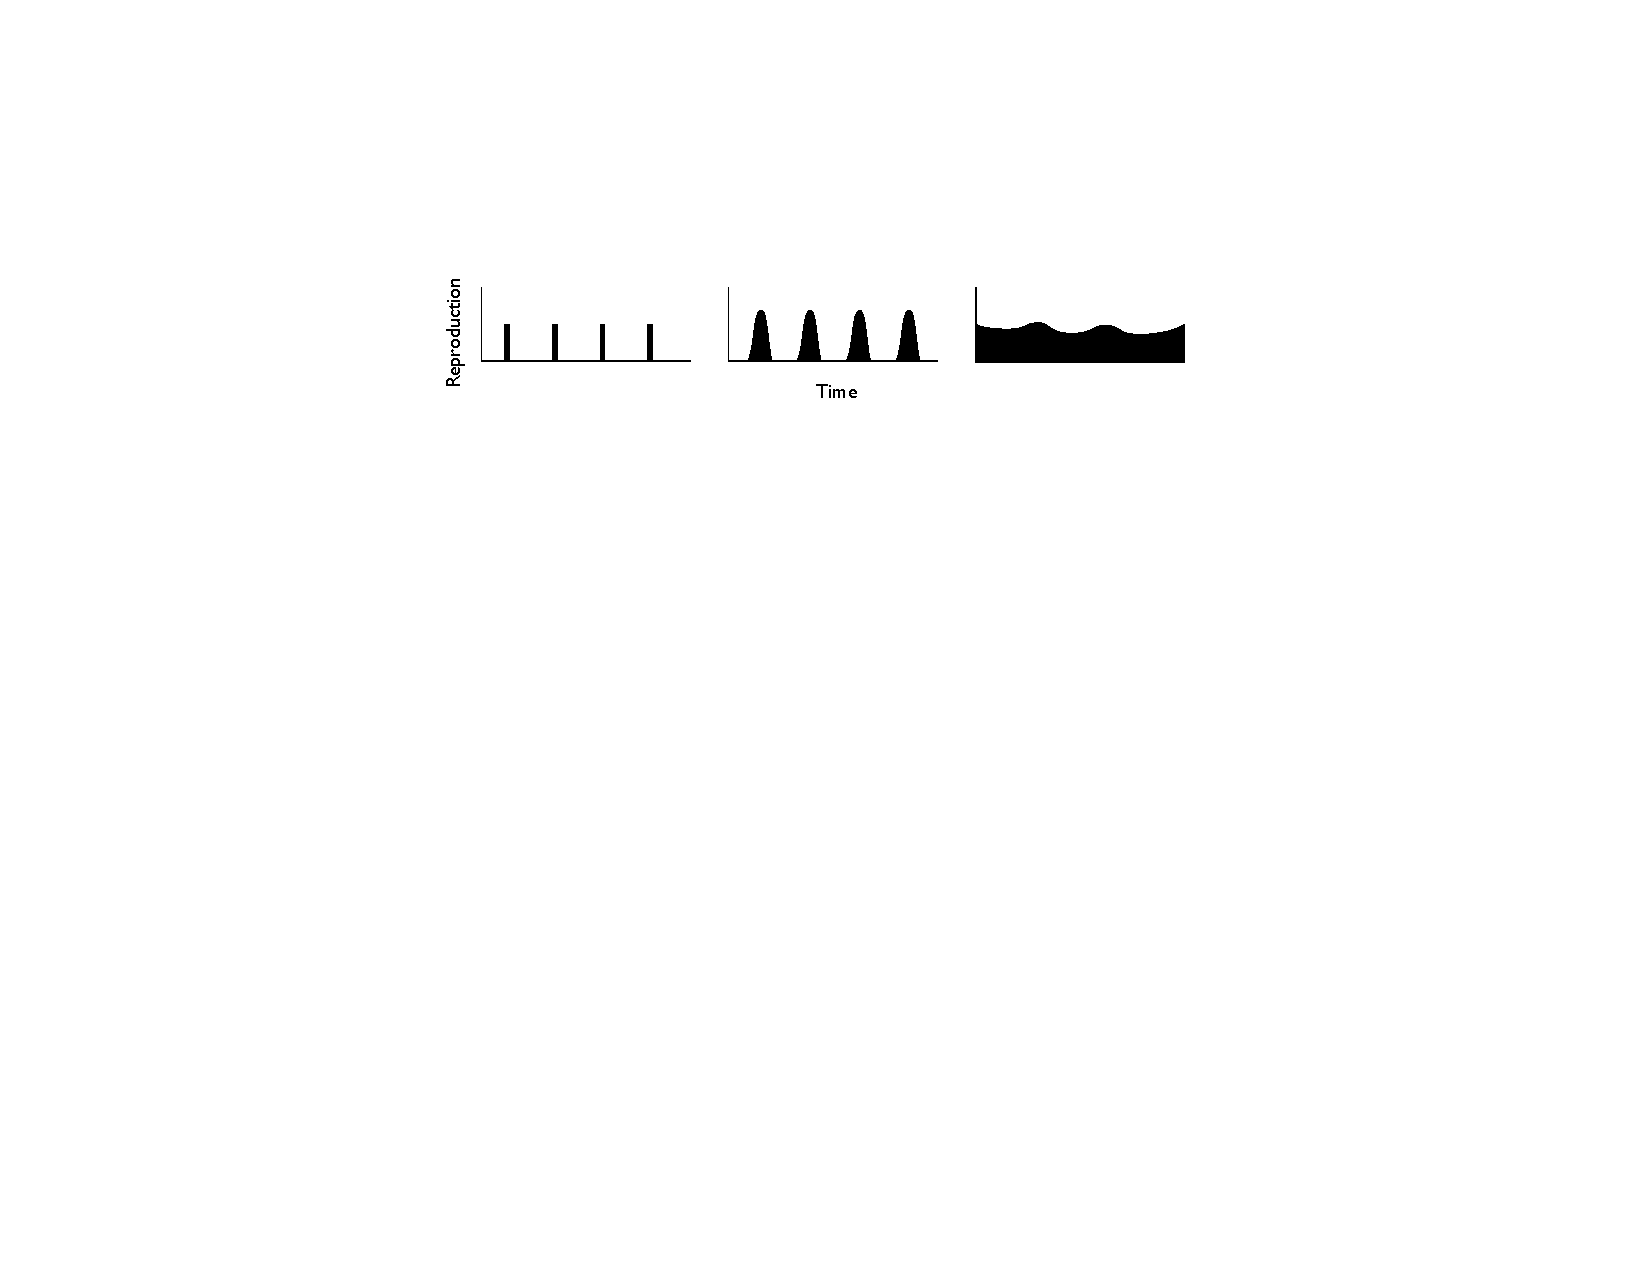
\includegraphics[width=8cm]{figs/image2}
\end{center}

Why emphasize this?\\
Empirical measurements of real populations are intrinsically discrete (we measure $N_0, N_1, N_2, ...$). Many empiricists therefore (inappropriately) default to discrete time models to estimate parameters like $\lambda$, even when biology of  species exhibits continuous growth on  time-scales being considered (for which estimating parameters like $r$ is appropriate for subsequent inferences).

\rule[0.5ex]{\linewidth}{1pt}

\circled{3}
How to get instantaneous population-level growth rate from projection equation, $N_0 e^{rt}$?\\
That is, how do we show that:
\begin{equation*}
\lim_{\Delta t \to 0}\left(\frac{\Delta N_t}{\Delta t}\right) = \frac{dN}{dt}
\end{equation*}

Need to take the derivative of $N_0 e^{rt}$ with respect to time $t$.  Use Product Rule:
\begin{equation*}
\frac{d(XY)}{dt}=\frac{d(X)}{dt}\cdot Y + X \cdot \frac{d(Y)}{dt}
\end{equation*}
\emph{``The derivative of a product is the sum of the product of the derivative of each term multiplied by the other term.''} Thus:
\begin{equation*}
\frac{d(N_0 \cdot e^{rt})}{dt}=\frac{d(N_0)}{dt}\cdot (e^r)^t + N_0 \cdot \frac{d((e^r)^t)}{dt}
\end{equation*}

Note:\\
\-\hspace{1cm} Derivative of a constant = 0\\
\-\hspace{1cm} Derivative of $a^x = ln(a)\cdot a^x$.

Thus:
\begin{align*}
	\frac{d(N_0 e ^{rt})}{dt} & =0 \cdot (e^r)^t + ln(e^r)\cdot (e^r)^t \cdot N_0\\
	&= r \cdot (e^r)^t \cdot N_0\\
	&= r \cdot e^{rt} \cdot N_0 \\
	&= r \cdot N_0 e^{rt} \\
\text{Since } N=N_0 e^{rt} \text{ for any time } t ...&\\
	&=rN=\frac{dN}{dt}
\end{align*}

\rule[0.5ex]{\linewidth}{1pt}

\circled{4}
Could also go in opposite direction from $\frac{dN}{dt} \rightarrow N_0 e^{rt}$:
\begin{align*}
&	\frac{dN}{dt}=rN\\
&	\frac{1}{N}\frac{dN}{dt}=r\\
&	\int_0^T \frac{1}{N}\frac{dN}{dt} \; dt = \int_0^T r\; dt \;\;\;\;(\text{Think of T as a constant, and t in dt as a variable})\\
&	\int_0^T \frac{1}{N}\frac{dN}{dt}  = r t \vert_0^T = r \cdot T - r \cdot 0\\
	\text{Using} \; \int \frac{1}{x}\; dx = ln(x)...\\
&	ln(N(T))-ln(N(0))=rT\\
& ln\left( \frac{N(T)}{N(0)}\right) = rT\\
& \frac{N(T)}{N(0)}= e^{rT}\\
& N(T)=N(0)e^{rT}
\end{align*}

\rule[0.5ex]{\linewidth}{1pt}

\break

Q for class: Qualitative analysis of population \emph{growth vs. decline}

\begin{center}
\begin{tabular}{|c|c|c|c|}
\hline \rule[-2ex]{0pt}{5.5ex} \emph{Population change} & $\lambda$ & $r_d$ &  $r$ \\ 
\hline \rule[-2ex]{0pt}{5.5ex} No change & 1 & 0 & 0 \\ 
\hline \rule[-2ex]{0pt}{5.5ex} Growth  & $>1$ & $>0$ & $>0$ \\ 
\hline \rule[-2ex]{0pt}{5.5ex} Decline & $<1$ & $<0$ & $<0$ \\ 
\hline 
\end{tabular}
\end{center} 

\note{Q:}  What are the units of $r$?
\note{A:} `Individuals \emph{per individual} per time'

\note{Q:}  What are the units of population growth rate, $\tfrac{dN}{dt}$?
\note{A:} `Individual per time'

\note{Q:}  What are the units of per capita growth rate, $\tfrac{1}{N}\tfrac{dN}{dt}$?
\note{A:} `Individuals \emph{per individual} per time'

\rule[0.5ex]{\linewidth}{1pt}

\textbf{Polynomial representation of $\frac{dN}{dt}$}

Recall: population size as function of time as polynomial
\begin{equation*}
	N(t)=\sum_{n=0}^\infty \beta_n t^n = \beta_0 + \beta_1 t + \beta_2 t^2 +...
\end{equation*}


Could also think of exponential growth as
\begin{align*}
&	\frac{dN}{dt}=f(N)=\sum_{n=0}^\infty \beta_n N^n \\
& 	\text{with } \beta_0=0, \;\; \beta_1 = r, \;\; \beta_{n>1}=0\\
\end{align*}
It's a `first-order' approximation.

\rule[0.5ex]{\linewidth}{1pt}

\note{Monod's nightmare}
\begin{align*}
&	t=20 \; min.,  \;\; N_t = 2N_0\\
&	N_t=N_0 e^{rt}\\
&	ln\left(\frac{N_t}{N_0}\right)=rt\\
&	ln(2)=rt\\
&	r=\frac{ln(2)}{t}=\frac{ln(2)}{20} \approx \frac{0.693}{20} = 0.035\% \text{ per minute}
\end{align*}


\rule[0.5ex]{\linewidth}{1pt}

\end{document}